{\color{teal!90}\chapter{Advanced configuration}\label{cap:advanced-configuration}}

\AddToShipoutPictureBG*{%
  \AtPageUpperLeft{%
    \raisebox{-\height}{%
      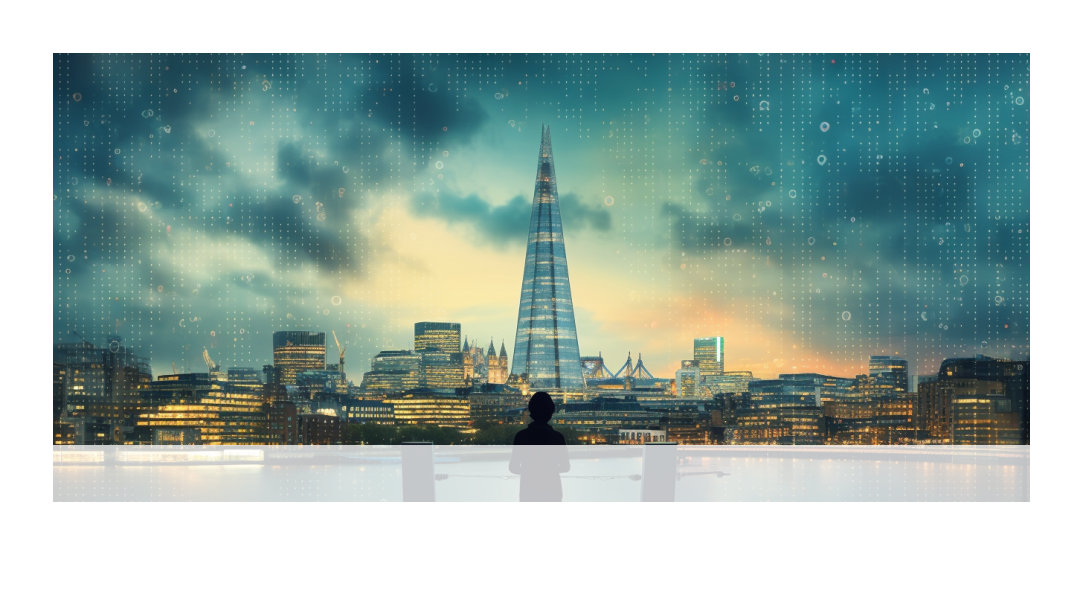
\includegraphics[width=\paperwidth]{./chapters/advanced-configuration.png}%
    }%
  }
}

\minitoc% Creating an actual minitoc mini lista contenuti


\section{Introduction}

In a context where we have configured an Android device in kiosk mode using the \gls{dpm} as a device owner, and we have implemented a custom launcher without access to settings for the end user, the action of setting up Termux and using its API to start Shizuku can be described as \emph{device preparation} or \emph{advanced configuration}

\medskip
\begin{center}
These actions \textbf{cannot} be considered {\color{BrickRed} \emph{a true privilege escalation}} in the traditional sense of the term
\end{center}
\medskip


This, is purely because we are configuring and using existing applications (Termux and Shizuku) to perform certain operations rather than gaining unauthorized or unintentional access at the system level. However, we are leveraging the features of Termux and Shizuku to perform advanced actions that would normally require root privileges or ADB commands. It's important to note that these actions should be clearly documented, and the device should be configured in compliance with company policies or device usage policies, especially considering its use in kiosk mode. Additionally, we should ensure that access to Termux and Shizuku is limited only to the necessary operations and that no security vulnerabilities are introduced that could compromise the stability or security of the kiosk device. In summary, while it's not a privilege escalation in the traditional sense, it is still an advanced device configuration that should be implemented carefully and appropriately documented.

For now we'll focus on the following actions:

\begin{itemize}
    \item Disabling keyboard and navigation overlays to make sure the device starts in a very protected state. The final user should never be able to use the terminal or navigate the device during boot sequence.
    \item Understanding what can we do with Shizuku now that is enabled. Why are they all claiming that Shizuku can call hidden APIs? How can we use them without having to use reflection?
    \item Use a service aware of the internal logcat to detect when termux is being launched so that we can start sending commands to it.
    \item Are there any termux commands that can be used to shut services down? For example, can we use termux to shut down the system UI?
    \item Can we make the gap shorter when we enable \gls{navisettings} temporarily? Can we make it so that it's only enabled for a few seconds?
    \begin{itemize}
        \item Can we actually have \gls{navisettings} enabled at all times and use Termux to make it secure?
    \end{itemize}
\end{itemize}